\documentclass[format=draft,degree=bachelor]{hustthesis}
% \usepackage{lua-visual-debug}

\stuno{U2009xxxxx}
\schoolcode{10487}
\title{\LaTeX 模板使用示例}{An Example of Using hustthesis \LaTeX{} Template}
\author{许铖}{Xu Cheng}
\major{电子信息工程}{Electronic and Information Engineering}
\supervisor{黑晓军\hspace{1em}副教授}{Ass. Prof. Xiaojun Hei}
\date{2013}{4}{1}

\zhabstract{
    这是一个\LaTeX{}模板使用实例文件,该模板用于华中科技大学毕业设计、学士论文、硕士论文和博士论文写作中。

    该模板基于LGPL 2.1发行。
}

\zhkeywords{\LaTeX{},华中科技大学,论文,模板}

\enabstract{
    This is a \LaTeX{} template example file. This template is used in written thesis for Huazhong Univ. of Sci. \& Tech.

    This template is published under LGPL 2.1 License.
}

\enkeywords{\LaTeX{}, Huazhong Univ. of Sci. \& Tech., Thesis, Template}

\begin{document}

\frontmatter
\maketitle
\makeabstract
\tableofcontents
\mainmatter

\chapter{基本格式测试}

\section{第一层}
\subsection{第二层}
\subsubsection{第三层}
测试测试测试测试测试测试测试测试测试测试测试测试。

\section{字体}

普通\textbf{粗体}\emph{斜体}

\hei{黑体}\kai{楷体}\fangsong{仿宋}

\section{公式}

单个公式,公式引用:公式\ref{eq:1}。
\begin{equation}
  E = mc^2 \label{eq:1}
\end{equation}

多个公式,公式引用:公式\ref{eq:2},公式\ref{eq:3}。

\begin{subequations}
\begin{equation}
  F = ma \label{eq:2}
\end{equation}
\begin{equation}
  c^2 = a^2 + b^2 \label{eq:3}
\end{equation}
\end{subequations}

\section{罗列环境}

\begin{enumerate}
    \item 第一层
    \item 第一层
    \begin{enumerate}
        \item 第二层
        \item 第二层
        \begin{enumerate}
            \item 第三层
            \item 第三层
        \end{enumerate}
    \end{enumerate}
\end{enumerate}

\begin{description}
    \item[解释环境]  解释内容
\end{description}

\chapter{其他格式测试}

\section{代码环境}

\begin{lstlisting}[language=python]
import os

def main():
    '''
    doc here
    '''
    print 'hello, world' # Abc
    print 'hello, 中文' # 中文
\end{lstlisting}

\section{定律证明环境}

\begin{definition}
这是一个定义。
\end{definition}
\begin{proposition}
这是一个命题。
\end{proposition}
\begin{axiom}
这是一个公理。
\end{axiom}
\begin{lemma}
这是一个引理。
\end{lemma}
\begin{theorem}
这是一个定理。
\end{theorem}
\begin{proof}
这是一个证明。
\end{proof}

\section{算法环境}

\begin{algorithm}[H]
\SetAlgoLined
\KwData{this text}
\KwResult{how to write algorithm with \LaTeX2e }
initialization\;
\While{not at end of this document}{
read current\;
\eIf{understand}{
go to next section\;
current section becomes this one\;
}{
go back to the beginning of current section\;
}
}
\caption{How to write algorithms}
\end{algorithm}

\section{表格}
表格见表\ref{tab:1}。

\begin{table}[ht]
\centering
\caption{一个表格}\label{tab:1}
\begin{tabular}{|c|c|}
\hline
a & b \\
\hline
c & d \\
\hline
\end{tabular}
\end{table}

\section{图片}
图片见图\ref{fig:1}。图片格式支持eps,png,pdf等。

\begin{figure}[hb]
\centering
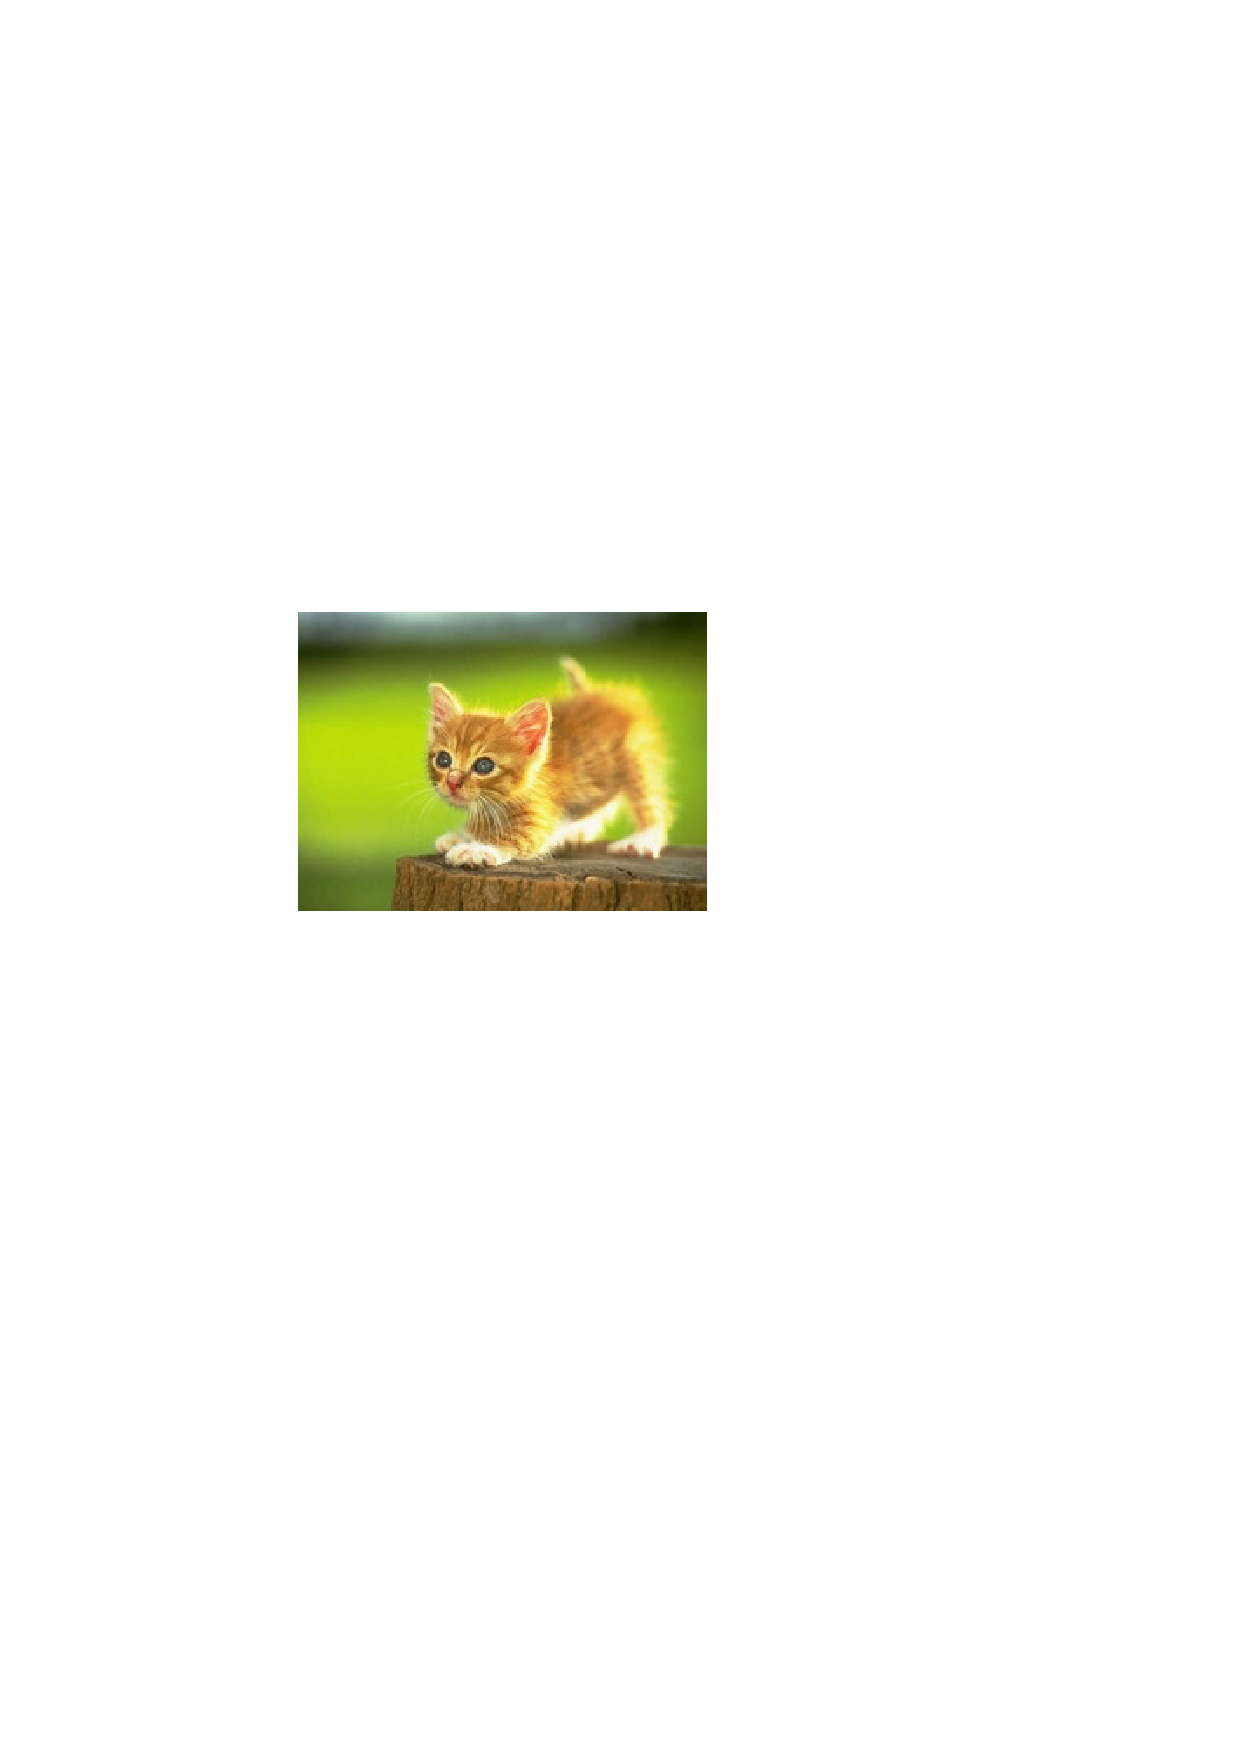
\includegraphics[width=.8\textwidth]{fig-example.pdf}
\caption{一个图片}\label{fig:1}
\end{figure}

\section{参考文献示例}
这是一篇中文参考文献\cite{TEXGURU99};这是一篇英文参考文献\cite{knuth};同时引用\cite{TEXGURU99,knuth}。

\backmatter

\begin{ack}
致谢正文。
\end{ack}

\bibliography{ref-example}

\listoffigures
\listoftables

\appendix

\begin{publications}
    \item 论文1
    \item 论文2
\end{publications}

\chapter{这是一个附录}
附录正文。

\end{document}